\documentclass{article}
\usepackage{graphicx} % Required for inserting images
\usepackage[margin=3cm]{geometry} % Adjust the margin as needed
\usepackage{tabularx}
\usepackage[table]{xcolor} % Pacchetto per colorare le celle
\usepackage[italian]{babel}
\usepackage{float}
\usepackage{hyperref}
\usepackage{caption}
\usepackage{subcaption}
\usepackage{listings}
\usepackage{amsmath}

\newcommand{\code}[1]{\texttt{#1}}

\title{Parallel Kernel Image Processing \\ \vspace{0.5cm} {Parallelizzazione e vettorizzazione di filtri di convoluzione su immagini}}
\author{Lorenzo Cappellini}
\date{Parallel Computing - A.A. 2025/2026}

\begin{document}

\maketitle

\newpage

\tableofcontents

\newpage
\section{Introduzione}

\subsection{Obiettivo}
Il progetto è stato sviluppato per l'assignment del corso di Parallel Computing, il quale richiede l'implementazione di un programma che sfrutti almeno uno degli approcci di parallelizzazione o vettorizzazione presentati durante il corso (OpenMP, vettorizzazione SIMD, CUDA), a partire da una versione sequenziale dello stesso algoritmo, corredata da un'analisi delle performance in termini di \textit{speedup}.
\\

\noindent Il problema scelto è il \textbf{Kernel Image Processing}, ovvero l'applicazione di un filtro di convoluzione 2D a un'immagine. Dato che ogni pixel in output è indipendente dall'altro, questa task si presta bene sia alla vettorizzazione SIMD che all'esecuzione parallela con OpenMP e su GPU.
\\

\noindent Il codice sorgente è disponibile su GitHub al seguente indirizzo:\\
\href{https://github.com/lcappellini/ParallelKernelImageProcessing}{https://github.com/lcappellini/ParallelKernelImageProcessing}.

\subsection{Kernel di convoluzione}
\label{subsec:theory}

La convoluzione 2D consiste nell'applicare a ciascun pixel dell'immagine una combinazione pesata dei pixel vicini, secondo una matrice di coefficienti detta appunto "Kernel". Dato un kernel di dimensione $K \times K$, il pixel di output è calcolato con la seguente formula:

\begin{equation}
    O(x,y) =
    \sum_{i=0}^{K-1}
    \sum_{j=0}^{K-1}
    I(x+i-r,\;y+j-r)\,K(i,j)
\end{equation}

\noindent dove $I$ rappresenta l'immagine di input, $K$ il kernel di convoluzione e $r = \lfloor K/2 \rfloor$ il raggio del kernel.
\noindent Per pixel appartenenti al bordo dell'immagine, le coordinate che fuoriescono dall'immagine vengono ricondotte al pixel di bordo più vicino (\textit{clamping}).
\noindent Assumendo una dimensione del kernel costante, il costo computazionale dell'algoritmo cresce linearmente con il numero $N$ di pixel dell'immagine, ovvero $O(N)$.

\noindent La convoluzione permette di realizzare diversi filtri d'immagine, tra cui \textit{sharpening}, \textit{gaussian blur}, \textit{edge detection kernel} ed \textit{embossing}. In questo progetto è stato utilizzato un kernel di \textit{edge detection}, applicato indipendentemente ai tre canali RGB.

\begin{figure}[H]
    \centering
    \begin{minipage}{0.49\textwidth}
        \centering
        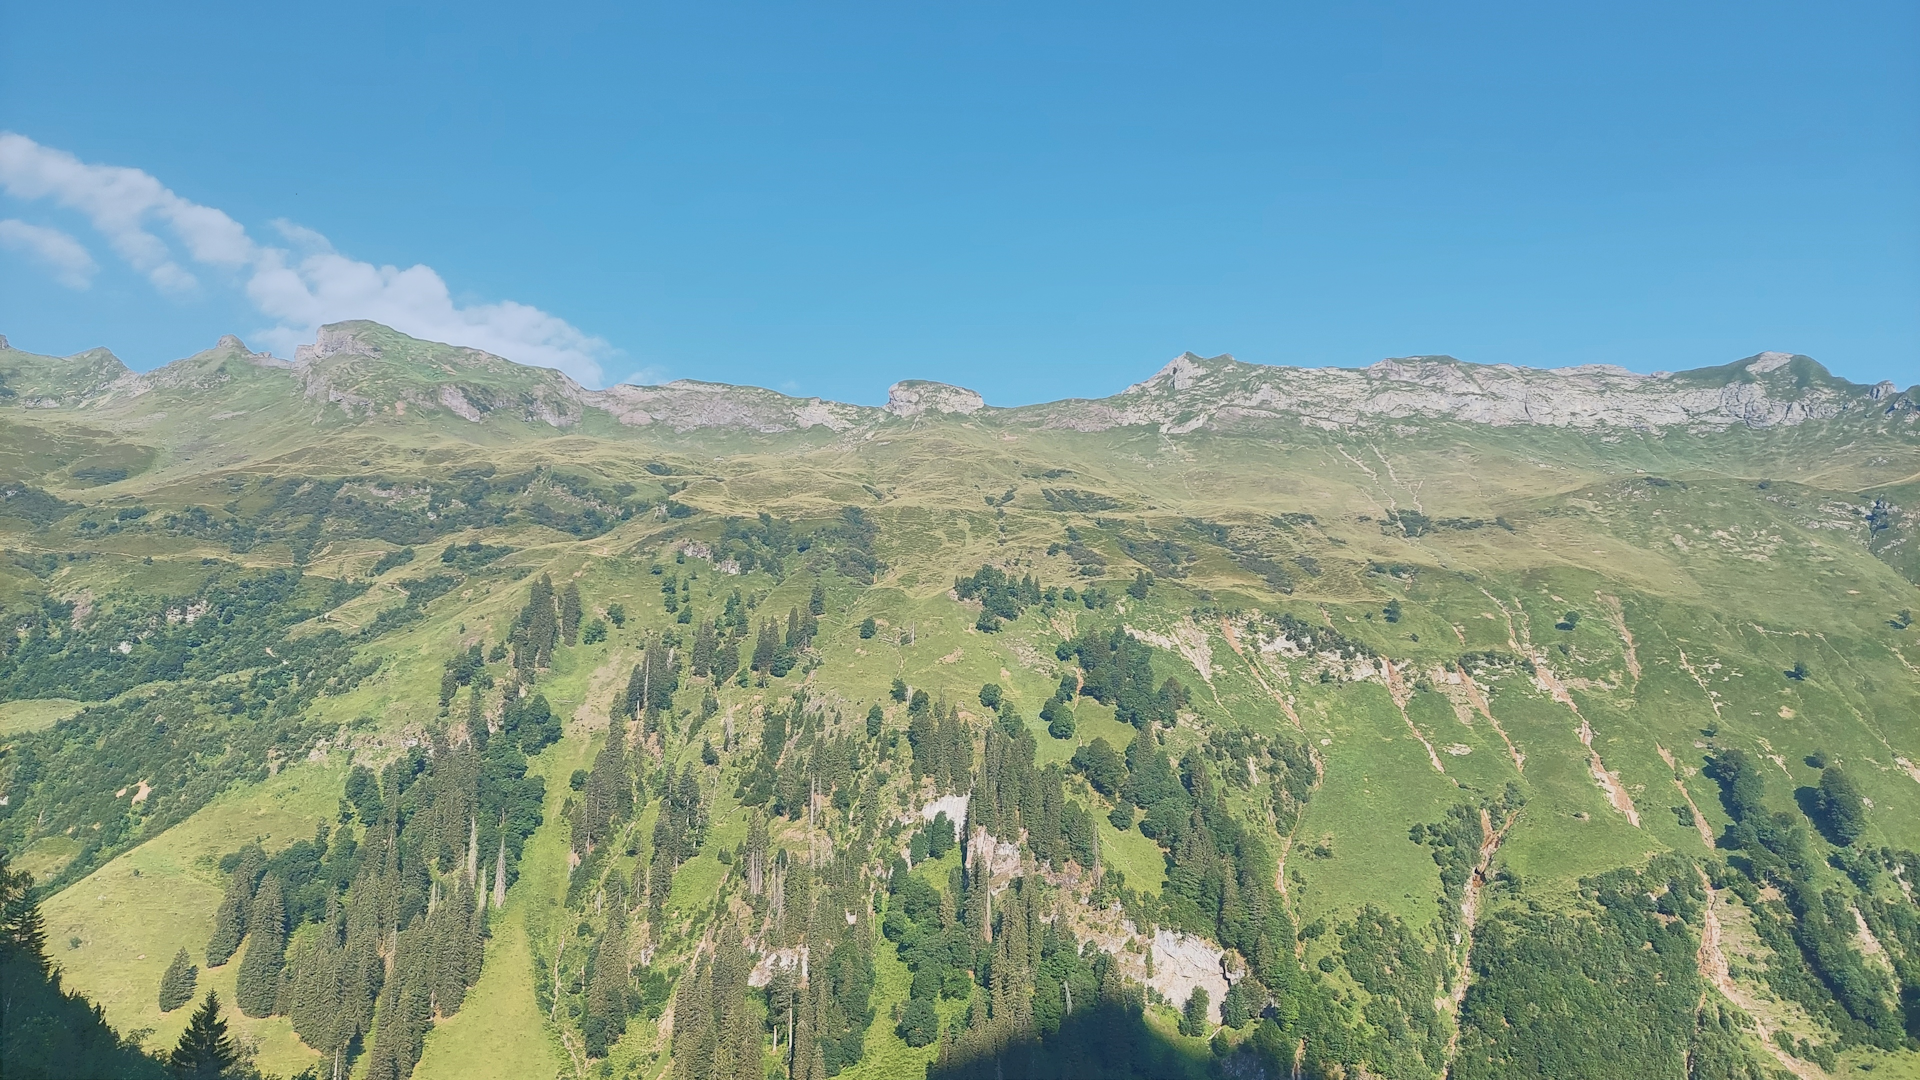
\includegraphics[width=\textwidth]{Graphs/Sample image.png}
        \caption{Immagine di partenza\newline}
        \label{fig:sample_image}
    \end{minipage}
    \begin{minipage}{0.49\textwidth}
        \centering
        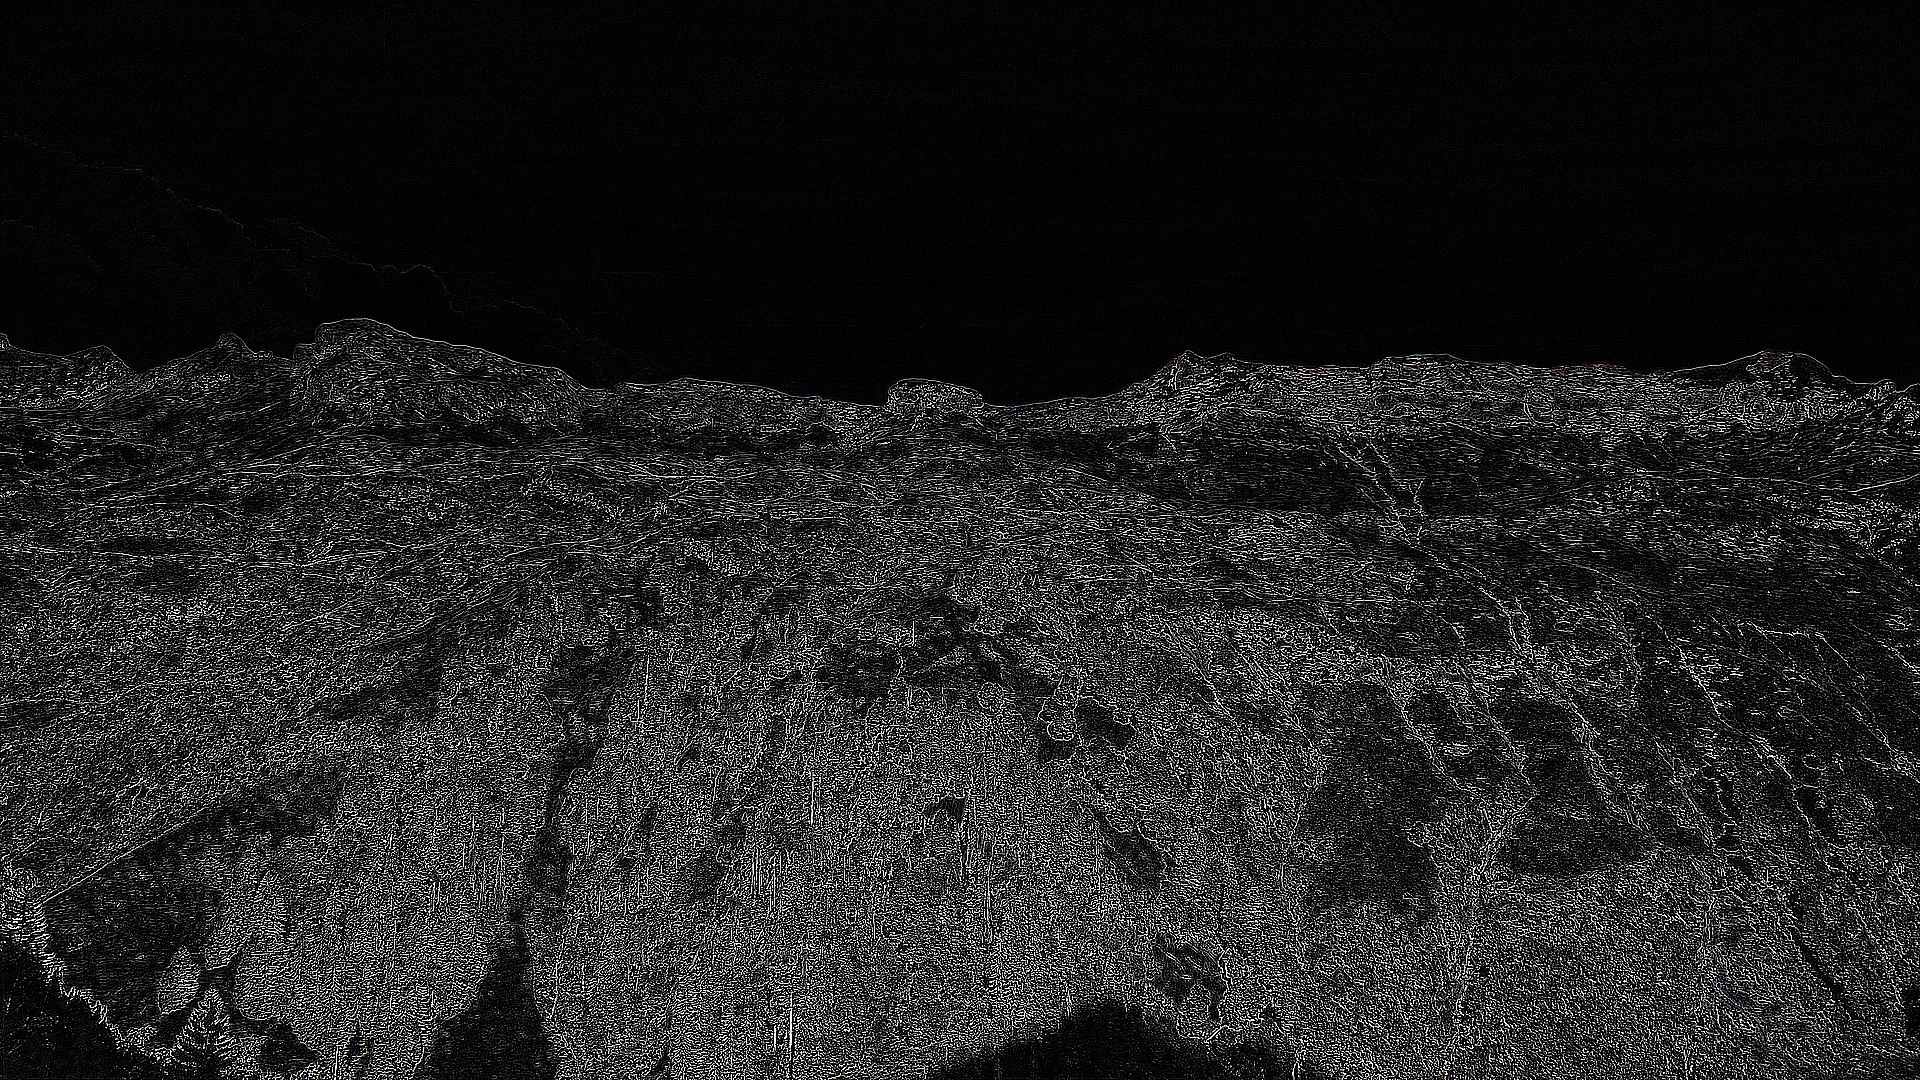
\includegraphics[width=\textwidth]{Graphs/Sample image fx.png}
        \caption{Immagine di output dopo l'applicazione del kernel di \textit{edge detection}}
        \label{fig:sample_image_fx}
    \end{minipage}
\end{figure}

\newpage

\subsection{Approcci utilizzati}
Sono state implementate e confrontate le seguenti configurazioni, tutte derivate dallo stesso algoritmo di convoluzione:

\begin{itemize}
    \item \textbf{Base}: versione sequenziale, quindi senza nessuna parallelizzazione né vettorizzazione esplicita.
    \item \textbf{OpenMP}: parallelizzazione su più thread del doppio ciclo sui pixel dell'immagine.
    \item \textbf{AVX2}: vettorizzazione delle istruzioni, che permette di eseguire quindi più operazioni con una singola istruzione.
    \item \textbf{OpenMP + AVX2}: combinazione delle due tecniche precedenti.
    \item \textbf{CUDA}: implementazione GPU con caricamento a tile in \textit{shared memory}.
    \item \textbf{AoS vs SoA}: confronto tra layout di memoria \textit{Array of Structures} e \textit{Structure of Arrays}. Entrambi sfruttano la vettorizzazione AVX2, al fine di valutare l'influenza del layout dei dati in memoria sull'efficienza della convoluzione vettorizzata.
\end{itemize}

\section{Implementazione}

\subsection{Flusso del programma}
Per ciascuna configurazione, il programma:
\begin{enumerate}
    \item carica tutte le immagini \code{.bmp} presenti nella cartella di lavoro con prefisso \code{in\_};
    \item per ciascuna immagine e ciascuna modalità di calcolo prevista, applica un filtro (in questo caso un kernel di \textit{edge detection});
    \item misura il tempo di esecuzione tramite \code{std::chrono::high\_resolution\_clock}; usando \\ \code{std::chrono::milliseconds} si ottenevano errori di troncamento troppo elevati relativamente a tempi di esecuzione troppo brevi (1-2 ms con CUDA), perciò è stato necessario utilizzare \code{std::chrono::microseconds} (nei grafici i tempi sono riconvertiti in ms);
    \item ripete l'esecuzione e la misurazione più volte (in questo caso 50), per ovviare ad eventuali fluttuazioni dovute ad altre task/processi del sistema operativo;
    \item salva le misurazioni su file \code{.csv}.
\end{enumerate}

\subsection{Classi}
\label{subsec:classi}
Per modellare il problema sono state create le seguenti classi:

\begin{itemize}
    \item \textbf{\code{Image}}: rappresenta un'immagine su cui operare e contiene dati come larghezza, altezza e numero di canali. Si occupa del caricamento e del salvataggio delle immagini (per semplicità è stato implementato soltanto il formato \code{.bmp}). L'immagine è salvata in layout \code{AoS} ed è possibile accedervi direttamente con un puntatore. Quando richiesto è possibile ottenere una copia convertita in layout \code{SoA}.
    \item \textbf{\code{Kernel}}: rappresenta il kernel di convoluzione, una matrice memorizzata come array lineare di float.
    \item \textbf{\code{ImageEditor}}: classe statica che implementa la logica di convoluzione vera e propria, in tutte le sue varianti. Espone metodi di applicazione diretta di effetti (come \code{edge\_detection\_effect}), che creano automaticamente i corrispettivo kernel e invocano il metodo \code{convolve} con la modalità richiesta (\code{AoS}, \code{SoA} o CUDA).
\end{itemize}

\subsection{Configurazioni}
Il programma è caratterizzato in più configurazioni diverse, perciò si ottengono di fatto più file eseguibili a sé stanti, ognuno compilato con precise flag di compilazione e ottimizzazione.

\subsubsection{Baseline sequenziale}
Questa configurazione è compilata senza direttive di parallelismo, e di fatto implementa in maniera sequenziale. Essa costituisce il riferimento base ($T_{seq}$) rispetto al quale vengono calcolati gli speedup delle altre versioni.

\subsubsection{Parallelizzazione con OpenMP}
In questa configurazione la parallelizzazione è ottenuta annotando il ciclo esterno sulle righe dell'immagine con \code{\#pragma omp parallel for}: ogni thread elabora un sottoinsieme di righe in modo da distribuire il carico di lavoro equamente.\\
\noindent Vista l'indipendenza dei pixel e delle operazioni, non c'è necessità di sincronizzazione tra i thread, operazione che rappresenta solitamente un notevole collo di bottiglia per le prestazioni.


\subsubsection{Vettorizzazione con AVX2}
La vettorizzazione AVX2 opera su gruppi di pixel adiacenti, applicando lo stesso coefficiente del kernel simultaneamente a più elementi tramite registri a 256 bit. Questo permette di eseguire la stessa operazione su più dati con una sola istruzione, riducendo quindi notevolmente i tempi di esecuzione.
Per questa configurazione la "conversione" delle normali operazioni in quelle SIMD è affidata al compilatore, specificando il flag \code{/arch:AVX2}.
\noindent È importante sottolineare che questo tipo di vettorizzazione deve essere supportata dalla CPU utilizzata (quasi tutte le CPU moderne).

\subsubsection{GPU computing con CUDA}
In questa configurazione, il programma, al posto della funzione di convoluzione \code{convolveAoS}, esegue una funzione che dopo aver preparato il device (GPU) e allocato la memoria necessaria, avvia l'esecuzione di un kernel CUDA.\\
\noindent In particolare l'implementazione CUDA (\code{convolution2DKernel\_2batch}) utilizza uno schema a \textit{tile} con \textit{shared memory}: ogni blocco di thread carica in memoria condivisa una porzione dell'immagine di input, allargata di un alone (\textit{halo}) pari al raggio del kernel, per poi calcolare i pixel di output del tile senza ulteriori accessi alla memoria globale. La dimensione del tile di output è fissata a $\text{TILE\_WIDTH}\times\text{TILE\_WIDTH}$ ed il blocco di thread lanciato ha la stessa dimensione del tile.

\noindent Dato che la zona da caricare (compreso l'\textit{halo}) è pari a $(\text{TILE\_WIDTH} + \text{Mask\_width} - 1)^2$, alcuni thread devono caricare due elementi in due fasi distinte {\textit{2-batch loading}}:
\begin{enumerate}
    \item \textbf{Primo caricamento}: ogni thread del blocco carica un primo elemento in \textit{shared memory}, calcolando le coordinate di destinazione a partire dall'indice del thread nel blocco.
    \item \textbf{Secondo caricamento}: gli stessi thread, con un offset pari alla dimensione del blocco, caricano un secondo elemento, necessario a coprire le celle di \textit{shared memory} non ancora riempite dalla prima fase. Solo i thread la cui destinazione ricade effettivamente dentro l'area di \textit{shared memory} eseguono questa seconda scrittura.
\end{enumerate}
In entrambe le fasi, le coordinate di input fuori dai limiti dell'immagine vengono gestite tramite \textit{zero-padding}: ai pixel esterni all'immagine viene assegnato valore zero.

\noindent Per ottenere un'ulteriore miglioria i puntatori all'immagine e alla mask sono dichiarati come \code{const \_\_restrict\_\_}: questo informa il compilatore che tali dati non vengono modificati durante l'esecuzione del kernel, in questo modo possono essere messi in una cache costante, velocizzando così i tempi di lettura.

\subsubsection{AoS vs SoA}
Per effettuare un confronto di prestazioni con la classica struttura dati in \code{AoS} (\code{RGBRGBRGB...}) usata per salvare i pixel delle immagini, la convoluzione è stata implementata anche con un approccio in \code{SoA}, quindi con i 3 canali colore divisi in 3 array diversi (\code{RRR...; GGG...; BBB...;}).
Come specificato nella sezione \ref{subsec:classi}, nel programma i pixel dell'immagine sono salvati con layout \code{AoS}, e convertiti in \code{SoA} prima della convoluzione. Dato che questa "traduzione" è separata dall'operazione di computazione principale e dipende esclusivamente dalla scelta implementativa di salvataggio dei dati che viene fatta, nella misurazione dei tempi di esecuzione non viene considerata.
Entrambe le implementazioni sono compilate con il flag \code{/arch:AVX2}, in modo da confrontare l'effetto del layout di memoria sulla vettorizzazione SIMD.

\section{Analisi delle performance}
\label{sec:performance}

\subsection{Setup hardware}
\renewcommand{\arraystretch}{1.4}
\begin{table}[H]
    \centering
    \begin{tabularx}{\textwidth}{ | l  X | }
        \hline
        \rowcolor{lightgray!70}
        \textbf{Componente} & \textbf{Modello} \\
        \hline
        CPU & AMD Ryzen 7 3700X 8-Core Processor\\
        \rowcolor{lightgray!40}
        RAM & 2 x Corsair 8GB DDR4\\
        GPU & NVIDIA RTX 3060 Ti\\
        \rowcolor{lightgray!40}
        Sistema operativo & Windows 10\\
        \hline
    \end{tabularx}
    \caption{Configurazione hardware/software utilizzata per i benchmark}
    \label{tab:hw_setup}
\end{table}


\noindent I grafici riportati nella Sezione \ref{sec:performance} sono stati generati a partire da questi file CSV tramite uno script Python dedicato.

\subsection{Metrica di valutazione}
\noindent Per confrontare tra loro le tecniche utilizzate, tutti i risultati ottenuti vengono espressi in termini di \textbf{speedup} rispetto alla configurazione sequenziale di base, oltre che di tempo assoluto. Lo speedup è definito come:
\begin{equation}
    S = \frac{T_{seq}}{T_{par}}
\end{equation}
dove $T_{seq}$ è il tempo impiegato dalla configurazione sequenziale Base e $T_{par}$ è il tempo impiegato dalla configurazione in analisi, a parità di dimensione dell'immagine in ingresso.\\
\noindent Ogni configurazione è stata eseguita $50$ volte su ogni immagine e dai tempi ottenuti è stato preso il valore mediano: questo permette di ottenere una misurazione più fedele che ignori le oscillazioni dovute allo scheduling delle altre task del sistema operativo.
\\

\newpage

\subsection{Dataset}

\noindent I test sono effettuati su immagini di dimensioni diverse, e rispecchiano le risoluzioni standard $16:9$. Queste sono generate a partire da una stessa immagine di partenza tramite uno script Python.\\
\noindent In questo modo è possibile valutare le prestazioni su un numero crescente di pixel (da $23$ mila a $130$ milioni).
\begin{table}[H]
    \centering
    \renewcommand{\arraystretch}{1.3}
    \begin{tabular}{ | l  c  r | }
        \hline
        \rowcolor{lightgray!70}
        \textbf{Nome} & \textbf{Risoluzione} & \textbf{Numero di pixel} \\
        \hline
        nHD & $640\times360$ & 230\,400 \\
        \rowcolor{lightgray!40}
        qHD & $960\times540$ & 518\,400 \\
        HD & $1280\times720$ & 921\,600 \\
        \rowcolor{lightgray!40}
        WXGA & $1366\times768$ & 1\,049\,088 \\
        HD+ & $1600\times900$ & 1\,440\,000 \\
        \rowcolor{lightgray!40}
        Full HD & $1920\times1080$ & 2\,073\,600 \\
        QHD & $2560\times1440$ & 3\,686\,400 \\
        \rowcolor{lightgray!40}
        4K UHD & $3840\times2160$ & 8\,294\,400 \\
        5K & $5120\times2880$ & 14\,745\,600 \\
        \rowcolor{lightgray!40}
        8K UHD & $7680\times4320$ & 33\,177\,600 \\
        16K UHD & $15360\times8640$ & 132\,710\,400 \\
        \hline  
    \end{tabular}
    \caption{Risoluzioni delle immagini utilizzate per i benchmark}
    \label{tab:resolutions}
\end{table}

\subsection{AoS vs SoA}

\begin{figure}[H]
    \centering
    \begin{minipage}{0.49\textwidth}
        \centering
        \fbox{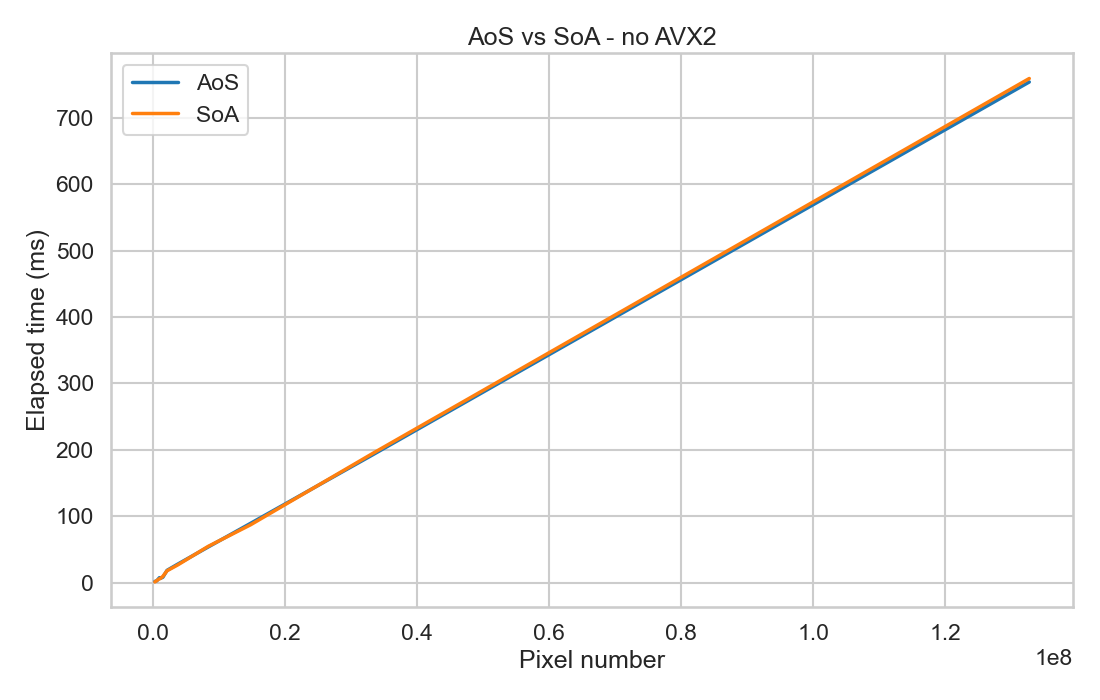
\includegraphics[width=0.9\textwidth]{Graphs/Graph AoS vs SoA no AVX2.png}}
        \caption{Tempi di esecuzione (ms) delle due implementazioni AoS e SoA, SENZA AVX2}
        \label{fig:graph_aos_vs_soa_no_avx2}
    \end{minipage}
    \begin{minipage}{0.49\textwidth}
        \centering
        \fbox{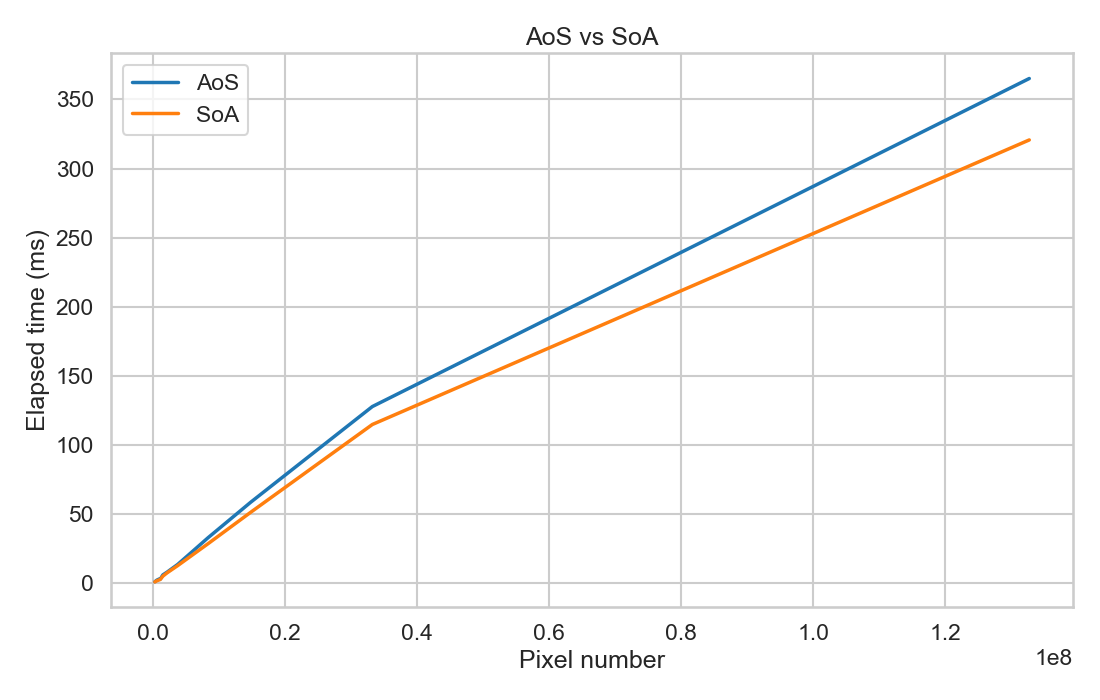
\includegraphics[width=0.9\textwidth]{Graphs/Graph AoS vs SoA.png}}
        \caption{Tempi di esecuzione (ms) delle due implementazioni AoS e SoA}
        \label{fig:graph_aos_vs_soa}
    \end{minipage}
\end{figure}

Il layout \code{SoA} è generalmente più favorevole laddove sono predominanti le operazioni sul singolo canale poiché i dati sono memorizzati in modo contiguo in memoria. Dunque, per questo problema specifico, la disposizione \code{SoA} in linea teorica non offre grandi vantaggi dato che l'operazione di convoluzione deve comunque essere eseguita su tutti i canali allo stesso modo.\\
Tuttavia con l'introduzione di AVX2, si nota una differenza: il layout \code{SoA} risulta più vantaggioso, poiché consente di caricare più efficientemente i valori dello stesso canale, dato che sono contigui in memoria. Nell'\code{AoS}, invece, i valori di uno stesso canale sono intervallati da quelli degli altri canali, rendendo necessarie operazioni di riordinamento aggiuntive.

\subsection{Confronto tempi di esecuzione}

\begin{figure}[H]
    \centering
    \begin{minipage}{0.49\textwidth}
        \centering
        \fbox{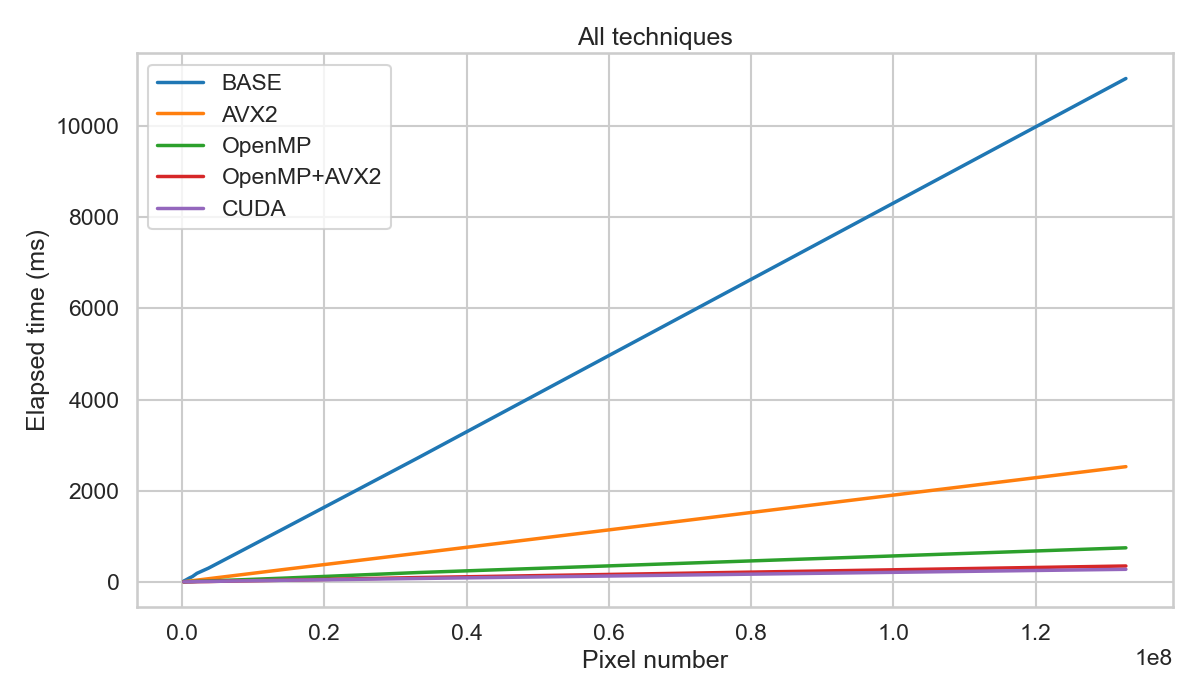
\includegraphics[width=0.9\textwidth]{Graphs/Graph All.png}}
        \caption{Grafico dei tempi impiegati da ogni configurazione}
        \label{fig:graph_times_all}
    \end{minipage}
    \begin{minipage}{0.49\textwidth}
        \centering
        \fbox{\includegraphics[width=0.9\textwidth]{Graphs/Graph All Bar.png}}
        \caption{Grafico a barre dei tempi impiegati da ogni configurazione (scala logaritmica)}
        \label{fig:graph_times_all_Bar}
    \end{minipage}
\end{figure}

Il grafico (\ref{fig:graph_times_all}) conferma che l'algoritmo di convoluzione ha costo $O(N)$, infatti il tempo di esecuzione cresce linearmente all'aumentare del numero di pixel per tutte le tecniche utilizzate. \\
\noindent Come pronosticabile, l'implementazione Base è la più lenta. Inoltre la suddivisione del carico su più thread (OpenMP) è comunque superiore alla vettorizzazione di AVX2 e la combinazione delle due tecniche consente di sfruttare entrambi i livelli di parallelismo, ottenendo prestazioni superiori. Per avere un'ulteriore miglioramento infine c'è CUDA, anche se con immagini piccole la differenza è praticamente nulla.


\subsection{Confronto Speedup}
\begin{figure}[H]
    \centering
    \fbox{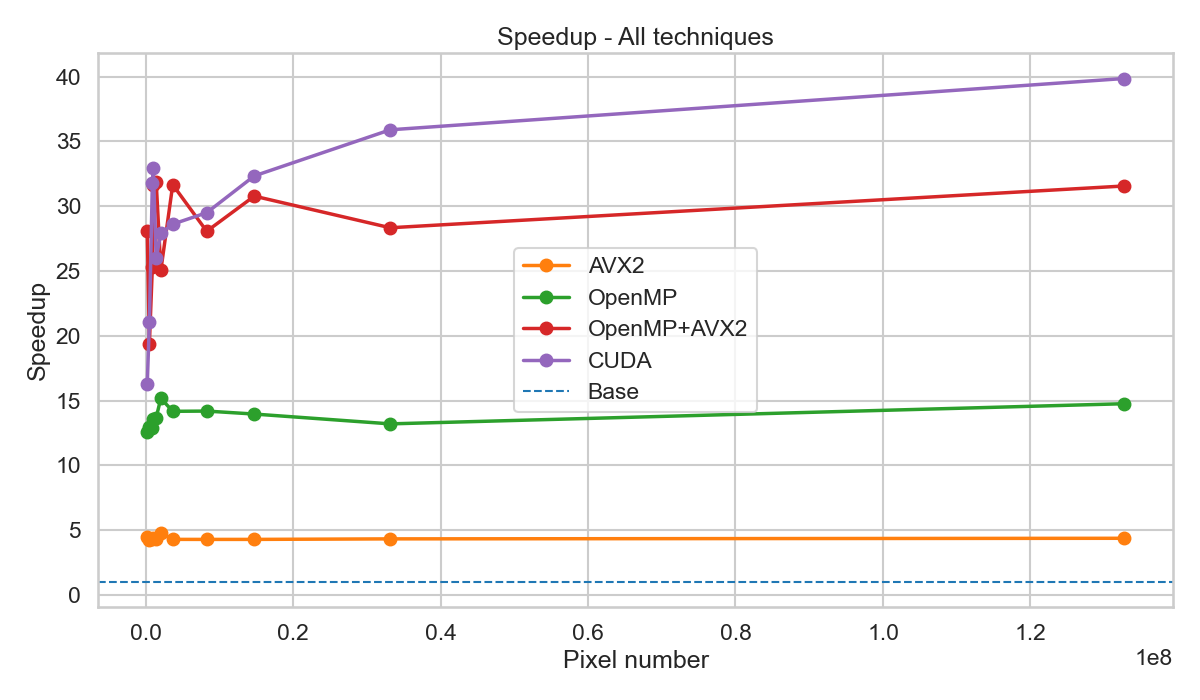
\includegraphics[width=0.8\textwidth]{Graphs/Graph All Speedup.png}}
    \caption{Grafico dei valori di speedup al variare del numero di pixel dell'immagine}
    \label{fig:graph_speedup_all}
\end{figure}

Tra tutti questo grafico è senza dubbio il più significativo in quanto permette di mettere a confronto visivamente il rendimento di ogni tecnica di parallelismo adottata e di analizzare il miglioramento che si ottiene. \\

\noindent Come per i tempi assoluti, anche qui l'andamento è piuttosto lineare, ma è interessante notare che:
\begin{itemize}
    \item per \textbf{AVX2} lo speedup è \textbf{costante}: eseguendo un certo numero (fisso) di operazioni in una sola, riduce il costo di ognuna di quel fattore, perciò lo speedup rimane tale anche al crescere dei pixel.
    \item per \textbf{OpenMP} lo speedup \textbf{cresce}: in questo caso sono presenti operazioni per creare il team di thread, scheduling e sincronizzazione della regione parallela; questo overhead ha un peso praticamente costante che si nota maggiormente quando lavora con un numero basso di pixel. Con un carico di lavoro superiore, la computazione stessa prevale, perciò l'\textbf{overhead diventa trascurabile}.
    \item per \textbf{CUDA} lo speedup ha un \textbf{andamento non lineare}: similmente a OpenMP, CUDA ha un \textbf{overhead}, ma molto più marcato a causa delle necessità di trasferimento dei dati tra host e device. Sono infatti indispensabili operazioni di allocazione (\code{cudaMalloc}), di copia (\code{cudaMemcpy}) e di "lancio" del kernel. Per quantità di dati minori (immagini piccole) il grande vantaggio della parallelizzazione sui thread della GPU viene quindi perso.
\end{itemize}

\noindent Per pixel count molto piccoli, sia CUDA che OpenMP+AVX2 mostrano grandi oscillazioni nello speedup, prima di stabilizzarsi su un andamento più regolare. Questo è dovuto al fatto che, a tempi di esecuzione dell'ordine del millisecondo, il rumore di misurazione ha un peso relativo molto più elevato rispetto al tempo di calcolo. Inoltre, dato che lo speedup è un rapporto tra due tempi, piccole variazioni assolute su $T_{par}$ si traducono in variazioni percentuali molto ampie sul risultato finale.

\section{Conclusioni}
Nella maggior parte dei casi il campo di applicazione tipico del Kernel Image Processing è quello dell'editing di immagini reali, acquisite da fotocamere, e le risoluzioni sono cresciute negli ultimi anni. Anche per questo motivo e visti anche i risultati ottenuti, l'approccio con \textbf{CUDA} è senza dubbio la \textbf{scelta più efficace}.
 
\noindent Anche le altre tecniche però non sono irrilevanti: CUDA richiede una \textbf{GPU NVIDIA}, che potrebbe non esser disponibile sui dispositivi; in questi contesti \textbf{OpenMP+AVX2} rappresenta l'alternativa più solida, con uno speedup comunque notevole, operando soltanto su CPU e \textbf{senza dispositivi hardware aggiuntivi}.
Anche \textbf{AVX2} da solo, pur con lo speedup più modesto, ha il vantaggio di richiedere \textbf{zero overhead} di setup ed essere applicabile senza coinvolgere altri thread, il che lo rende una scelta ragionevole quando la parallelizzazione \textbf{multithread non è praticabile}.

\end{document}